\chapter{Some Disassembly Required} 
\label{sec:disassembly}
\lstset{style=6502Style}

We've reached the point where the game has started to execute. We just saw a
snippet of code that turned off the tape recorder and prompted the C64 to run a
routine\index{routine} called \icode{MainControlLoop\index{MainControlLoop}}.
Though perhaps a little cryptic, and you shouldn't expect to understand it yet,
this code is not exactly what the machine 'saw'. Instead it read and executed
something far more puzzling-looking:


\begin{lstlisting}[caption=The first piece of machine code that is executed in Iridis Alpha.,escapechar=\%]
78A9 408D 1903 A900 8D18 03A9 108D 04DD A900 8D05
DDA9 7F8D 0DDD A981 8D0D DDA9 198D 0EDD 584C 3508 
\end{lstlisting}

That's right it executed a stream of bytes. A stream of bytes commonly referred to as \textit{machine code}. Each of these
bytes is meaningful to the C64 whether individually, or taken in pairs, or even in groups of three. It can comprehend them
as instructions to carry out that will shuffle data around in its memory and ultimately result in a game that
can be played.

Before we can dig into the internals of how Iridis Alpha works we have to convert all of the machine code we've
loaded into memory in the previous chapter into something we have a chance of reading and understanding. This
process is called disassembly and here we're going to explain how it is done and along the way gain a little
basic understanding of the human-readable language, called '6502 Assembly Language', that we convert the machine
code back into.

The process is called \textit{disassembly} simply because it is the exact reverse of the process that was originally followed
to generate the data on the tape from the assembly language written by Jeff Minter in the first place. Programs that
do this are referred to as 'assemblers'. They assemble the instructions written by the programmer into machine code
that the C64 can execute. As self-appointed disassemblers we are going to turn it back into assembly language.

\begin{definition}[Jeffrey Says]
\setlength{\intextsep}{0pt}%
\setlength{\columnsep}{3pt}%
\begin{wrapfigure}{l}{0.12\textwidth}
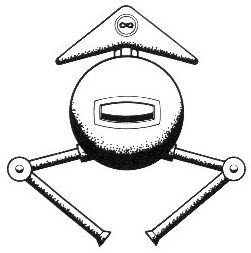
\includegraphics[width=\linewidth]{src/callout/ia.jpg} 
\end{wrapfigure}
\small

According to Jeff Minter's development diary, Iridis Alpha was programmed and "assembled
on a C128 using a partially-finished JCL assembler and the horrible, slow
Commodore disk drives." 
You've read that correctly: Iridis Alpha was not written
on a C64 but its more powerful and expensive, and hence much less popular, successor
the C128. 

\begin{figure}[H]
  {
    \begin{adjustbox}{width=7cm,center}
      \frame{\surface{disassembly/jcl.png}}
    \end{adjustbox}
  }\caption[]{The 1984 JCL Assember on the C128. You can imagine how user-friendly this thing must have been.}
\end{figure}
This wasn't so uncommon back in the day: computers like the C64 were not
powerful enough for getting any actual work done (such as writing and assembling a game),
so the programming and assembling was done on more capable, but often prohibitively expensive,
microcomputers. As long as the assembler was configured to output a file that could be run on
the C64, actual development could be done on any system the developer found tolerable. Or as
  Minter put it: "Next time I'm gonna use a 6502 X-ASM running in 2.5 Megabytes of RAM on 
  me trusty [Atari] ST..."
\end{definition}

Along the way we will have to invent names for things that are meaningful to us: the names Jeff Minter gave to his
functions, routines, and variables are long since lost to us. They were thrown away by the assembler as unnecessary
for execution of the machine code. As we proceed, we will see why but it hopefully makes sense to say that the
6502 CPU in the C64 doesn't care what things are called it just cares where in the 65,632 bytes of its RAM things
are located. That is to say it only cares about their 'address'.

So let's start by stepping back for a second. Let's put the machine code and the snippet of code we disassembled it
back into and see what we can learn:

\begin{minipage}[b]{0.45\linewidth}
\centering
\lstinputlisting[caption=Machine Code]{disassembly/bytes.asm}
\end{minipage}
\hspace{0.5cm}
\begin{minipage}[b]{0.45\linewidth}
\centering
\lstinputlisting[caption=Assembly Language]{disassembly/disassembled-bytes.asm}
\end{minipage}


Straightaway we can infer meanings to some of the bytes:

\begin{figure}[H]
  {
    \setlength{\tabcolsep}{3.0pt}
    \setlength\cmidrulewidth{\heavyrulewidth} % Make cmidrule = 
    \begin{adjustbox}{width=3cm,center}

      \begin{tabular}{rllllllll}
        \toprule
        Byte & Instruction &\\
        \midrule
78 & SEI & \\
A9 & LDA & \\
8D & STA & \\
58 & CLI & \\
4C & JMP & \\
        \addlinespace
        \bottomrule
      \end{tabular}
    \end{adjustbox}
  }\caption{Machine code bytes and their assembly language counterparts.}
\end{figure}

Let's quickly explain what two of these mean as they're extremely common and also fundamental to
machine code programming in general.

\icode{LDA} loads the byte you give it into a small one-byte slot called the 'Accumulator' ('A' for short,
so \icode{LDA} is an abbreviation for 'Load to Accumulator'). Think of this slot
as a pocket - somewhere for the CPU to store a value for use later on. The technical name for this kind of 
slot/pocket is a 'register\index{register}'. The 'Accumulator' is so-called because a lot of the operations performed on
bytes stored in this particular pocket have very precise behaviour when addition operations are executed on
it. But we never really have to worry about this too often and in the general case it is simply used, as
here, as a place to put a value so we can do something else with it.
\clearpage

\begin{lstlisting}[caption=Loading the byte \$40 to the \icode{Accumulator}.,escapechar=\%]
LDA #$40
\end{lstlisting}

What we do with it for the most part in the code above is go on to store it somewhere else. This is where
the \icode{STA} instruction comes in. This stores the value in the 'Accumulator' pocket at the address
in memory that you give to it. As we can see such addresses are not one byte long, but two bytes. Are they
ever more than two bytes long? No, and for a very simple reason. The C64 can only understand addresses
that are at most two bytes long and this is what ultimately limits it to 64KB of memory. The largest address it can understand
is therefore \icode{\$FFFF} - the largest value that can be expressed by 2 bytes. Which translates to 65,535.
Including zero, this allows us 65,536 bytes, which is 64KB of RAM. 

When we look at the disassembly of the STA instructions we see something quite puzzling:

\begin{minipage}[b]{0.45\linewidth}
\centering
\begin{lstlisting}[escapechar=\%]
8D 19 03
\end{lstlisting}
\end{minipage}
\hspace{0.5cm}
\begin{minipage}[b]{0.45\linewidth}
\centering
\begin{lstlisting}[escapechar=\%]
STA $0319
\end{lstlisting}
\end{minipage}

Shouldn't we have expected \icode{8D 19 03} to translate to \icode{STA \$1903} rather than 
\icode{STA \$0319}? Why are the numbers back to front like that? The reason is due to something
you may have heard described with a word that you've never fully understood and maybe never
dared to question. The machine code
stores the address \icode{0319} as \icode{1903} because the 6502 CPU in the C64 expects to read
addresses with the second half of the number first. When we read numbers we expect it to start
with the most significant digits first, i.e. \icode{\$0319}. But most computer architectures of the 1980s had the opposite
expectation - reading the least significant digits first, or the least significant bits first since
this is a computer we're talking about, i.e. \icode{\$1903}. This approach possesses a couple of advantages,
the main one being that the computer can start performing an operation on the number (e.g. addition) before it
has read all of it. For example, if you're adding 5312 and 2043 you already have enough to get started with once
you've read 12 and 43. The carrying etc. can all happen once you've read the rest of the two numbers. This approach
is known as `little-endian' byte ordering. The opposite, which is closer to what we are familiar with when
reading numbers ourselves, is called `big-endian'. If you had never heard of either of those terms before, then
you have now.

The next incremental step in understanding our disassembly is to apply some meaning to these two-byte values
that we've decoded. As it happens, all the ones given in this piece of code represent addresses in the C64's
memory of \icode{\$FFFF} bytes, or in the preferred parlance of we humans, 65,536 bytes. Each address here
has a particular function\index{function} so storing a value in it does something. Let's add the meanings, which are still
a little cryptic, to our listing:

\begin{minipage}[b]{0.20\linewidth}
\centering
\lstinputlisting[title=Assembly]{disassembly/disassembled-bytes.asm}
\end{minipage}
\hspace{0.5cm}
\begin{minipage}[b]{0.70\linewidth}
\centering
\lstinputlisting[title=Assembly Language with some comments]{disassembly/labelled-bytes-1.asm}
\end{minipage}

As you may remember we said in the previous chapter that this little routine\index{routine} is doing two things: the first
is telling the C64 to jump to and execute the routine\index{routine} that starts the actual game the next time it 'wakes up'; the
other thing it's doing is turning off the cassette tape reader so that no more data is read from the tape.

The bit that's turning off the tape reader is this:

\begin{lstlisting}[escapechar=\%]
LDA #$10
STA $DD04    ;CIA2: Timer A: Low-Byte%\index{Low-Byte}%
LDA #$00
STA $DD05    ;CIA2: Timer A: High-Byte%\index{High-Byte}%
LDA #$7F
STA $DD0D    ;CIA2: CIA Interrupt%\index{Interrupt}% Control Register%\index{Register}%
LDA #$81
STA $DD0D    ;CIA2: CIA Interrupt%\index{Interrupt}% Control Register%\index{Register}%
LDA #$19
STA $DD0E    ;CIA2: CIA Control Register%\index{Register}% A
\end{lstlisting}

We are better off treating this series of instructions as a magic formula. The operation of the tape reader
is managed by the values stored in a series of bytes between \icode{\$DD04} and \icode{\$DD0F}. The fact that
we have to write a variety of values to 5 of them to just stop reading from the tape is just a testament
to the power of boring overhead - we'll never interact with the tape reader again so studying the entrails
here is not going to benefit us in any way.

The other thing this routine\index{routine} is doing - preparing the C64 to execute the game proper - is more compact and
introduces two concepts that are going to be important throughout our tour of the Iridis Alpha code so it
is worth spending some time on them here to get them clear.

\begin{lstlisting}[caption=Containing two important concepts.,escapechar=\%]
LDA #$40
STA $0319    ;Non-Maskable Interrupt%\index{Interrupt}%
LDA #$00
STA $0318    ;Non-Maskable Interrupt%\index{Interrupt}%
\end{lstlisting}

\section{Important Concept Number One: High Bytes and Low Bytes}
On the face of it these four instructions are doing something very simple. They are storing the value \$40
at address \$0319 and the value \$00 at \$0318. What they are actually doing is storing the address \$4000
in a place where the C64's 6502 CPU will be expected to look in a moment's time and take that as a command
to start executing whatever is at address \$4000.


\begin{figure}[H]
  {
    \setlength{\tabcolsep}{3.0pt}
    \setlength\cmidrulewidth{\heavyrulewidth} % Make cmidrule = 
    \begin{adjustbox}{width=7cm,center}
      \begin{tikzpicture}
        \draw[step=1.0,gray,thin] (0,0) grid (8,2);
        \fill[gray] (3,1) rectangle ++ (2,1);
        \node[matrix of math nodes,anchor=south west,inner sep=0pt,
              nodes={draw,minimum size=1cm,anchor=center},
              column sep=-\pgflinewidth,row sep=-\pgflinewidth,font=\ttfamily]
              {
\icode{43} & \icode{36} & \icode{34} & \icode{00} & \icode{40} & \icode{41} & \icode{50} & \icode{45} \\
\icode{0315} & \icode{0316} & \icode{0317} & \icode{0318} & \icode{0319} & \icode{031A} & \icode{031B} & \icode{031C} \\
						  };
      \end{tikzpicture}
    \end{adjustbox}
  }\caption{The slice of C64 memory between addresses \$0315 and \$031C and the bytes that live there after we've
written \icode{\$40} to \icode{\$0319} and \$00 to \$0318.}
\end{figure}

The reversed order we spoke about earlier, the 'little-endian' order, in which the 6502 CPU stores and reads
pairs of bytes is observed again here. When the CPU reads the contents of \icode{\$0318} and \icode{\$0319}
it interprets them not as \icode{\$0040}, which is the order in which they appear to us, but as \icode{\$4000}.

When discussing this storage arrangement we refer to the contents of \icode{\$0318} as the 'Low Byte' and the
contents of \icode{\$0319} as the `High Byte'. `High' is just another way of saying 'first', and 'Low' another
way of saying `second'. When taking about a values like \icode{\$4000} stored in \icode{\$0318-\$0319} such as in this case \icode{\$40} is the
'High Byte' and \icode{\$00} is the 'Low Byte'.

Writing values to a pair of adjacent addresses in memory like this so that they can
be subsequently interpreted as yet another address to get something from or do something with is a very common
pattern\index{pattern} in programming 6502 CPUs such as the C64's and we will encounter it a \textit{lot} in this book.

It's a strange sort of indirection when you first attempt to understand it. Instead of storing actual values
at an address, we're storing an \textit{address} in the address. If you are familiar with other programming languages
you may already recognize this concept and understand how powerful it can be. If you are not it will probably
seem strange and maybe even wasteful. Seeing the many uses it is put to in the Iridis Alpha code may persuade
you otherwise, but hopefully when we look at the use it is put to here you may begin to get a flavor of its
utility. Let's do that by looking at our second important concept.

\section{Important Concept Number Two: Interrupts}
\begin{lstlisting}[caption=It's an interrupt\index{interrupt}. And it's non-maskable.,escapechar=\%]
LDA #$40
STA $0319    ;Non-Maskable Interrupt%\index{Interrupt}%
LDA #$00
STA $0318    ;Non-Maskable Interrupt%\index{Interrupt}%
\end{lstlisting}

We previously\index{previously} waved away what's happening in this code by saying that the address \icode{\$4000} will be interpreted
as an address to jump to and start executing the next time the 6502 CPU 'wakes up'. That's a lot of hand-waving.

The technical term for this 'waking up' is an 'interrupt\index{interrupt}'. This waking up happens incredibly frequently, 60 times every second.
60 times a second the C64 will stop what it's doing and execute whatever is given as an address by the bytes at \icode{\$0318-\$0319}.

The number 60 may ring a bell for you in this context. A common aspiration for graphics\index{graphics}-based games, and minimum table-stakes today,
is that a game runs at 60 'frames per second'. In other words, that at least 60 times a second the display is updated and whatever
is on the screen\index{screen} moves a little bit.

While a C64 programmer would never achieve 60 frames per second in practice, 'interrupts' are the C64's mechanism for at least
getting some of the way there. They allow the game developer to at least do something to the display many times per second.
Whatever it is, it has to be something short and sweet and at the same time effective enough to actually progress the gameplay.
This is why this concept is important to us: most of the important things that happen in Iridis Alpha will be effected during
an interrupt\index{interrupt}. When we look at moving, shooting, and blowing things up, all of them are going to happen in routines that are called
multiple times per second by the 6502 CPU executing the code that has been stored at the address \icode{\$0318-\$0319} at that
point in time.

And this is our first taste of the power of storing an address in an address. Depending on where we are in the game - be it the
title screen\index{screen}, the main game, the bonus phase, or in a pause mode sub-game, the code that we want to run during these interrupts
will be different.

We can see this in action if we look at what happens when the code at \icode{\$4000} is executed. We've given this address \icode{\$4000}
a 'label' name of \icode{MainControlLoop\index{MainControlLoop}} in our disassembled code so \icode{MainControlLoop\index{MainControlLoop}} always refers to whatever lives at
\icode{\$4000}. 

\begin{lstlisting}[caption=The code at \icode{\$4000}. ,escapechar=\%]
MainControlLoop%\index{MainControlLoop}%
        LDA #$00
        SEI
p4003   LDA #<MainControlLoopInterruptHandler%\index{MainControlLoopInterruptHandler}%
        STA $318    ;NMI
        LDA #>MainControlLoopInterruptHandler%\index{MainControlLoopInterruptHandler}%
        STA $319    ;NMI
\end{lstlisting}

As you can see the first thing it does is change the address of the code that should be executed at every 'interrupt\index{interrupt}'. It's now an
address referred to by the label \icode{MainControlLoop\index{MainControlLoop}\-InterruptHandler}. This happens to be address \icode{\$6B3E} but the beauty
of using labels in our code is that we no longer need to worry about the number of the addresses anymore. The label will do the job
for us. It does mean we have to know what the syntax \icode{\#<MainControlLoopInterruptHandler\index{MainControlLoopInterruptHandler}} means though. What it means is:
if \icode{MainControlLoopInterruptHandler\index{MainControlLoopInterruptHandler}} lives at \icode{\$6B3E} the \icode{\#<} decorators refer to the \icode{\$3E} part of the
address, so we're actually saying \icode{LDA \#\$3E}, i.e. load the value \icode{\$3E} into the 'Accumulator'. Similarly the syntax
\icode{\#>MainControlLoopInterruptHandler\index{MainControlLoopInterruptHandler}} refers to the \icode{\$6B} part of the address.

\begin{figure}[H]
  {
    \setlength{\tabcolsep}{3.0pt}
    \setlength\cmidrulewidth{\heavyrulewidth} % Make cmidrule = 
    \begin{adjustbox}{width=7cm,center}
      \begin{tikzpicture}
        \draw[step=1.0,gray,thin] (0,0) grid (8,2);
        \fill[gray] (3,1) rectangle ++ (2,1);
        \node[matrix of math nodes,anchor=south west,inner sep=0pt,
              nodes={draw,minimum size=1cm,anchor=center},
              column sep=-\pgflinewidth,row sep=-\pgflinewidth,font=\ttfamily]
              {
\icode{43} & \icode{36} & \icode{34} & \icode{3E} & \icode{6B} & \icode{41} & \icode{50} & \icode{45} \\
\icode{0315} & \icode{0316} & \icode{0317} & \icode{0318} & \icode{0319} & \icode{031A} & \icode{031B} & \icode{031C} \\
						  };
      \end{tikzpicture}
    \end{adjustbox}
  }\caption{The values in \icode{\$0318} and \icode{\$0319} after we've updated them in \icode{MainControlLoop\index{MainControlLoop}}.}
\end{figure}

We've almost squeezed as much as we can out of this short and boring snippet of code. There's just one last thing to point
out that will be useful to us later. The last instruction in the routine\index{routine}:

\begin{lstlisting}[caption=Jump.,escapechar=\%]
JMP $0835
\end{lstlisting}

This tells the CPU to jump to the address \$0835 and execute whatever is there. What is at \icode{\$0835}? This:

\begin{lstlisting}[caption=Hello again.,escapechar=\%]
JMP $0835
\end{lstlisting}

That's right - it's jumping\index{jumping} back to itself and will execute in an infinite loop repeatedly executing the instruction
over and over again. The reason it does this is because it won't be doing it very long. The interrupt\index{interrupt} will take over
and steal execution away so that the C64 can find better things to do that run in circles.

Before we move on let's take one last look at our disassembly accomplishment.

\lstinputlisting[caption=Fully disassembled]{disassembly/labelled-bytes-2.asm}

Hopefully with these basics under our belt we can begin to understand how the interesting parts of Iridis Alpha work.
